\thispagestyle{empty}
\begin{center}
\vspace*{0.5in}

{\Huge\bfseries\color{skdark} MATHLIB5}\\[0.2in]
{\Large\bfseries\color{skmid} An Immutable System of Safety Boundaries\\[0.05in]
for Verified Symbolic Compute}\\[0.35in]

\noindent\rule{0.7\textwidth}{1.5pt}\\[0.25in]

{\large\color{skblue} The Verified Symbolic Compute Pipeline (VSCP)}\\[0.1in]
{\normalsize\color{skgray} A Ten-Layer Architecture for Auditable,\\[0.02in] Provenance-Sealed Symbolic Mathematics}\\[0.5in]

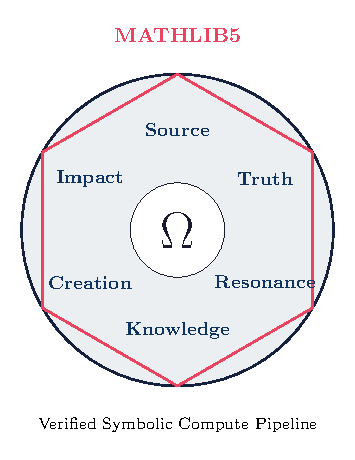
\includegraphics[width=0.45\textwidth]{figs/pipeline_diagram.pdf}\\[0.5in]

{\large\bfseries Ahmad Ali Parr}\\[0.08in]
{\normalsize SnapKitty Collective \textperiodcentered\ SNAPKITTYWEST}\\[0.08in]
{\normalsize Saint Errant Digital Society}\\[0.3in]

{\normalsize\color{skgray} Draft Research Monograph \textperiodcentered\ July 2026}\\[0.1in]
{\small\color{skgray} ORCID: 0009-0006-1916-5245}\\[0.1in]
{\small\color{skgray} Repository: \url{https://github.com/SNAPKITTYWEST/mathlib5}}

\vfill

\begin{tcolorbox}[skcallout,title=Provenance Anchor]
\textbf{Manuscript fingerprint (SHA-256):}\\
\ttfamily\tiny \input{anchors/fingerprint.txt}\\
\textbf{Ed25519 public key:}\\
\ttfamily\tiny \input{anchors/pubkey.txt}\\
\textbf{Bitcoin OP\_RETURN anchor:}\\
\ttfamily\tiny \input{anchors/opreturn.txt}
\end{tcolorbox}

\end{center}
\clearpage
